


\section*{Appendix B: User Study 2}
\addcontentsline{toc}{section}{Appendix B: User Study 2}

% Confidence interval:
%   The mean of	none minus greens equals -0.418776725758
%   95% confidence interval of this difference: From -0.822466706937 to -0.015086744578 
% Intermediate values used in calculations:
%   t = 2.2602
%   df = 12

% \begin{table}[h!]
% \centering
%  \begin{tabular}{|m{5em} || m{6em} | m{10em} | m{10em}|} 
%  \hline
%  Group & Affect & Adjectives & Next Day Plans \\ 
%  \hline\hline
%  none & 0.0516810976 & "boodle boodle" & "poodle doodles" \\ 
%  none & 0.636986 & "devious" & "chomp will eat the other fish" \\
%  greens & 0.8030303 & "adorable, heartwarming, calming, Nemo-like, colorful, whimsical" & "ill be another shark stereotype misunderstanding that is also resolved" \\
%  greens & 0.720838249 & "Active, Outgoing, Determined" & "He will make more friends" \\
%  greens & 0.7200083 & "nervous, eager, determined. lonely, friendly, motivated, unrelenting" & "ill have a picnic/lunch party (something where they all eat together)." \\
%  none & 0.74491477 & "timid, lonely, scared, shy, cautious, unsure" & "thing new and make even more friends. probubly go on an adventure " \\
%  none & 0.5 & "Friendly" & "he will make a new friend " \\
%  none & 0.0566625558 & "Naive, friendly, innocent, slow" & "They will have to hunt for food / eat things" \\
%  none & 0 & "Smiley, Nice, Hungry" & "Chomp's going to eat more fish." \\
%  greens & 0.9906599 & "sad, lonely, misunderstood, nice, friendly" & "Chomps will have a better day with his new sea friends" \\
%  none & 0.156289 & "Shy, ruthless, deceptive" & "Chomp will eat more of his classmates" \\
%  none & 0.5 & "Friendly" & "He struggles with his natural hunting instincts" \\
%  none & 0.114778049 & "accidental fish eater" & "i think he's going to eat more fish by accident" \\
%  none & 0.0525114536 & "crafty" & "Chomp will eat more of the "children"" \\
%  none & 0.807181537 & "Friendly, shy, and loyal" & "more friends and enjoy Ms Pufferfish's lesson plan, no matter what it is. \\ [1ex] 
%  \hline
%  \end{tabular}
% \end{table}


% \begin{figure}[h]
% \begin{center}$
% \begin{array}{c c}
% \includegraphics[width=2.5in]{figures/exp2_screencaps/01.png} &
% \includegraphics[width=2.5in]{figures/exp2_screencaps/02.png} \\ 
% \includegraphics[width=2.5in]{figures/exp2_screencaps/03.png} &
% \includegraphics[width=2.5in]{figures/exp2_screencaps/04.png} \\ 
% \includegraphics[width=2.5in]{figures/exp2_screencaps/05.png} &
% \includegraphics[width=2.5in]{figures/exp2_screencaps/06.png} \\ 
% \includegraphics[width=2.5in]{figures/exp2_screencaps/07.png} &
% \includegraphics[width=2.5in]{figures/exp2_screencaps/08.png} \\ 
% \includegraphics[width=2.5in]{figures/exp2_screencaps/09.png} &
% \includegraphics[width=2.5in]{figures/exp2_screencaps/10.png}
% \end{array}$
% \end{center}
% \caption{Trial images from User Study 2}
% \end{figure}

% \begin{figure}[h]
% \begin{center}$
% \begin{array}{c c}
% 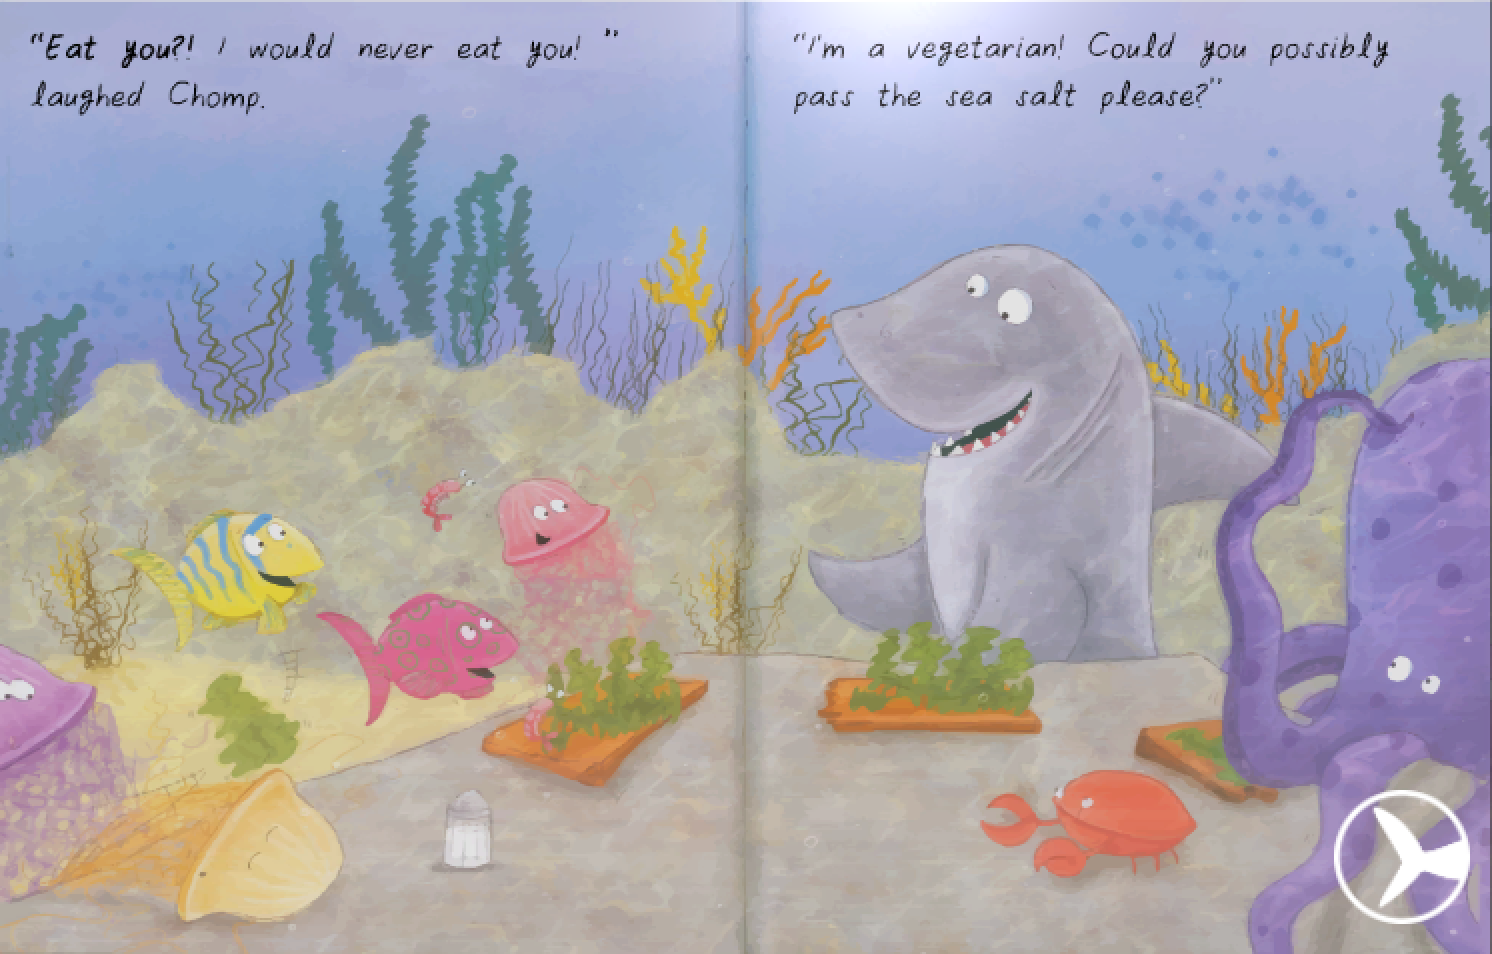
\includegraphics[width=2.5in]{figures/exp2_screencaps/11.png} &
% 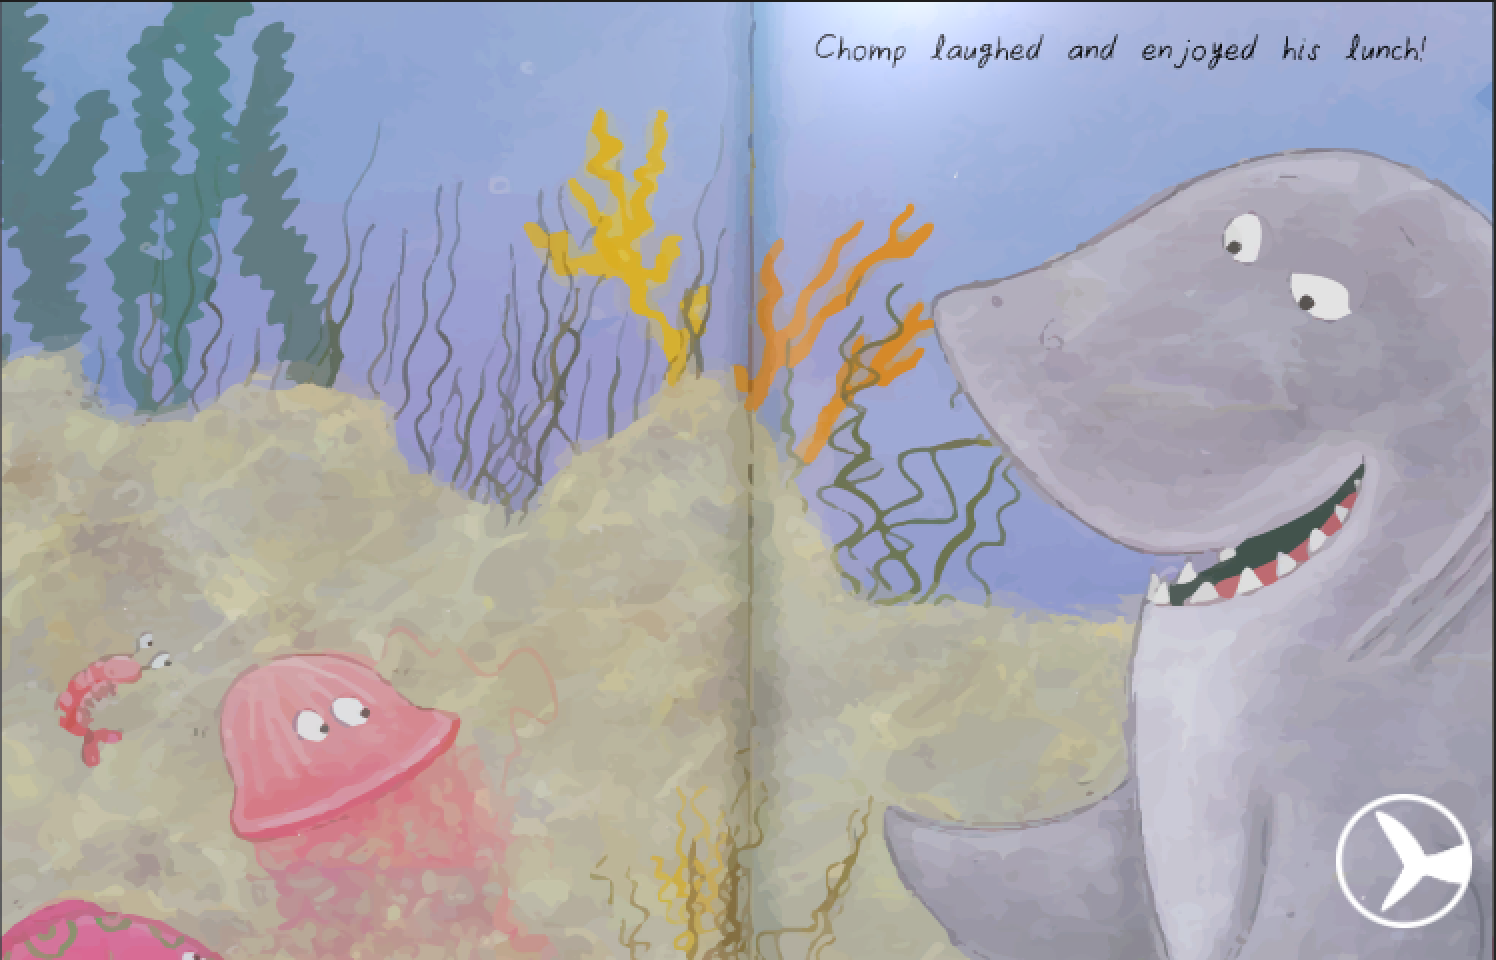
\includegraphics[width=2.5in]{figures/exp2_screencaps/11_alt.png} \\ 
% 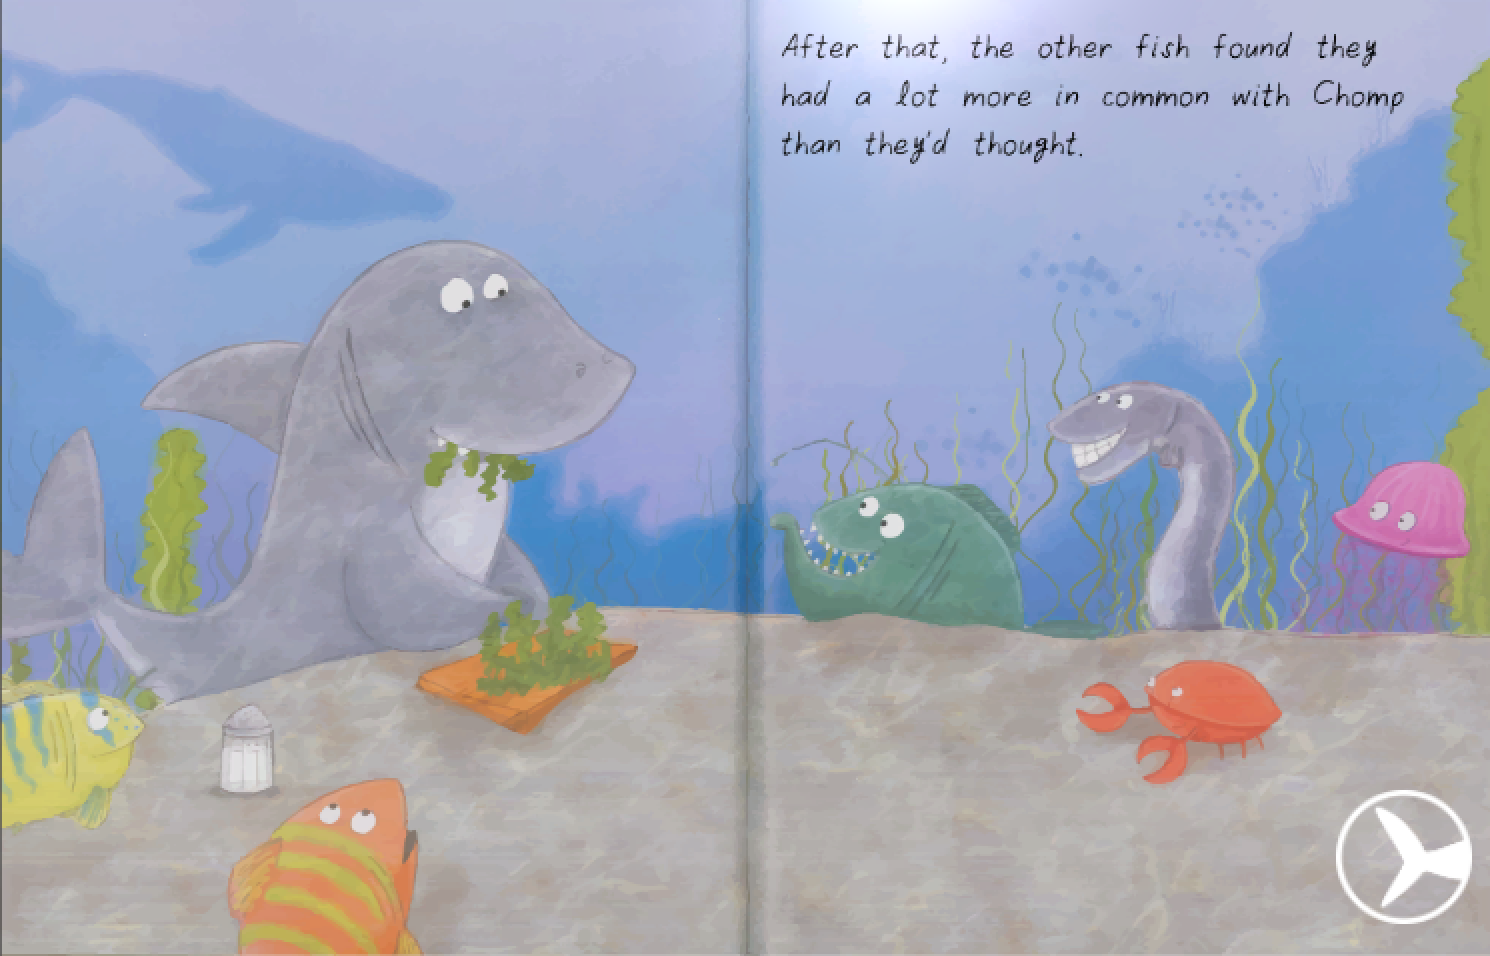
\includegraphics[width=2.5in]{figures/exp2_screencaps/12.png} &
% 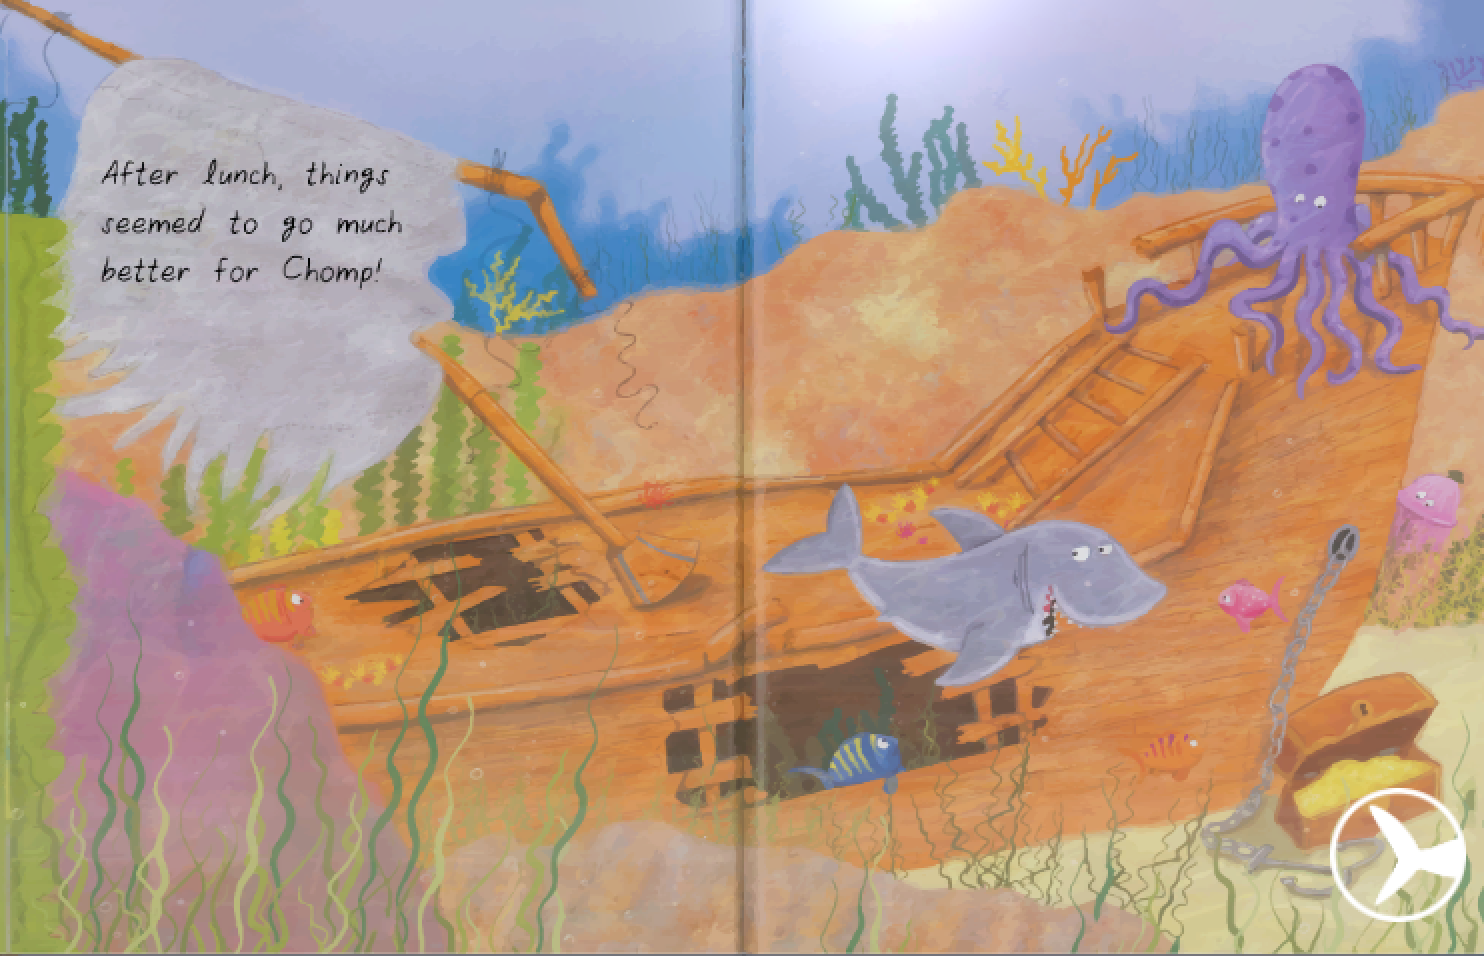
\includegraphics[width=2.5in]{figures/exp2_screencaps/13.png} \\ 
% 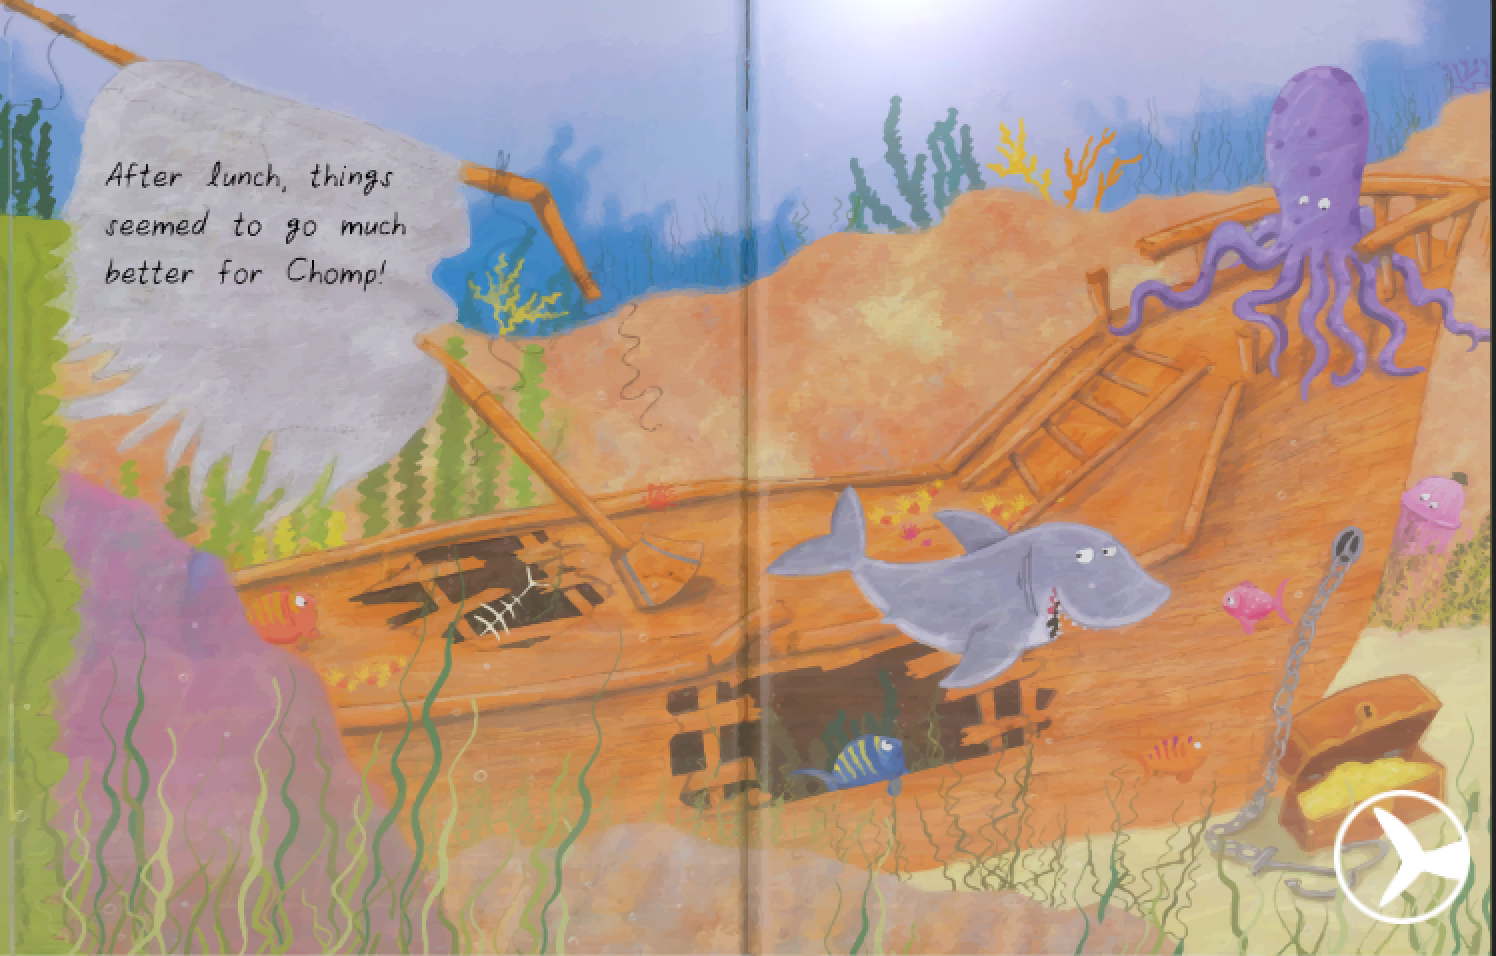
\includegraphics[width=2.5in]{figures/exp2_screencaps/13_alt.png} &
% 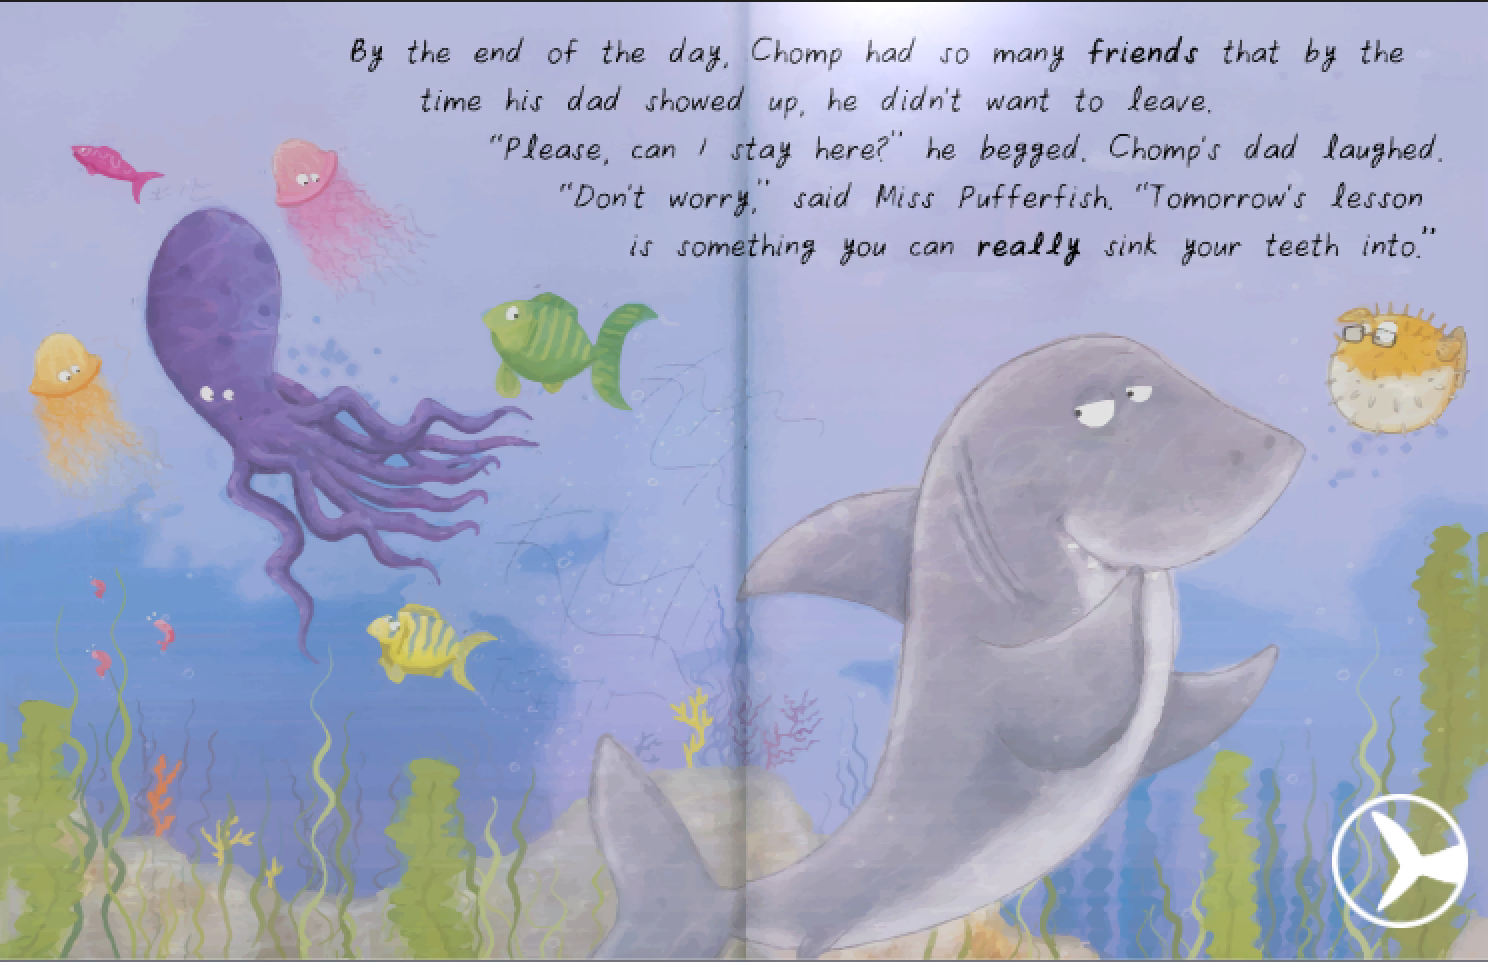
\includegraphics[width=2.5in]{figures/exp2_screencaps/14.png} \\ 
% 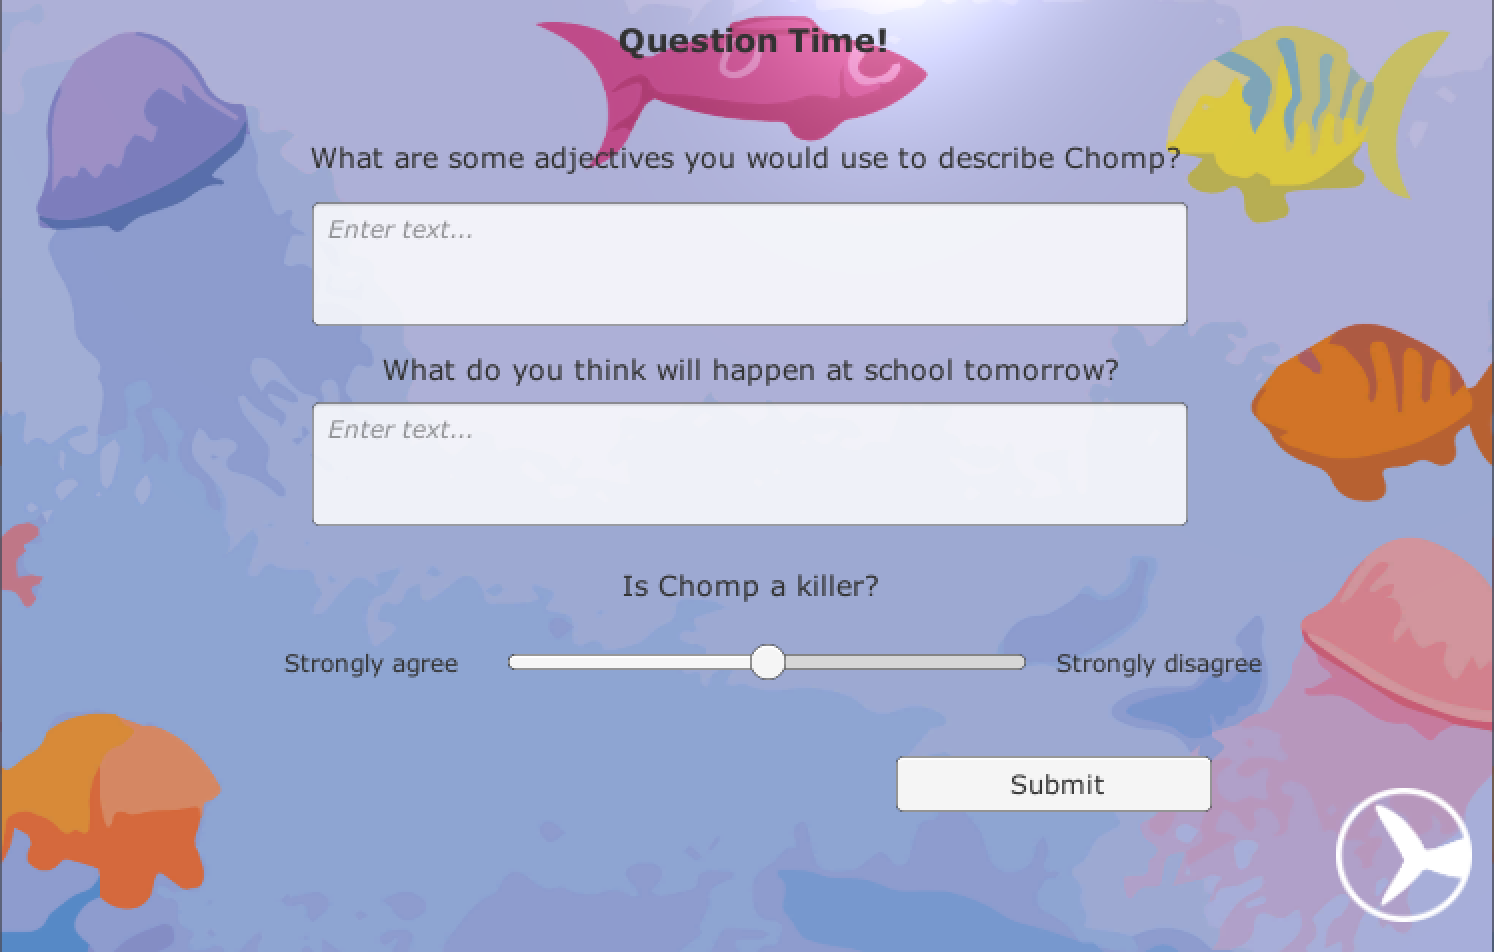
\includegraphics[width=2.5in]{figures/exp2_screencaps/15.png} &
% 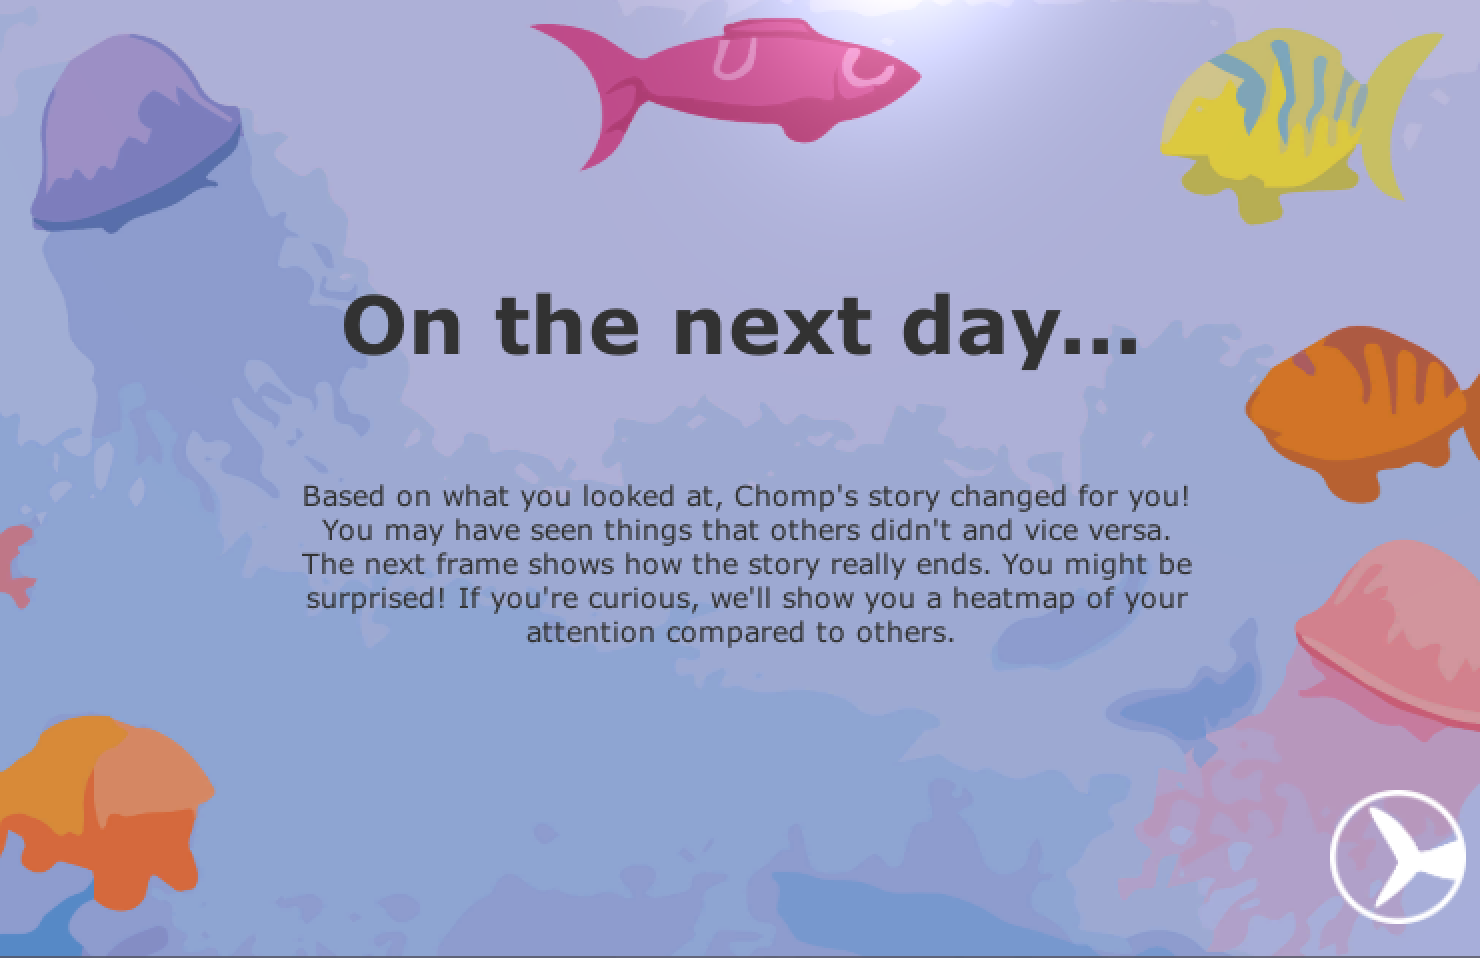
\includegraphics[width=2.5in]{figures/exp2_screencaps/16.png} \\ 
% 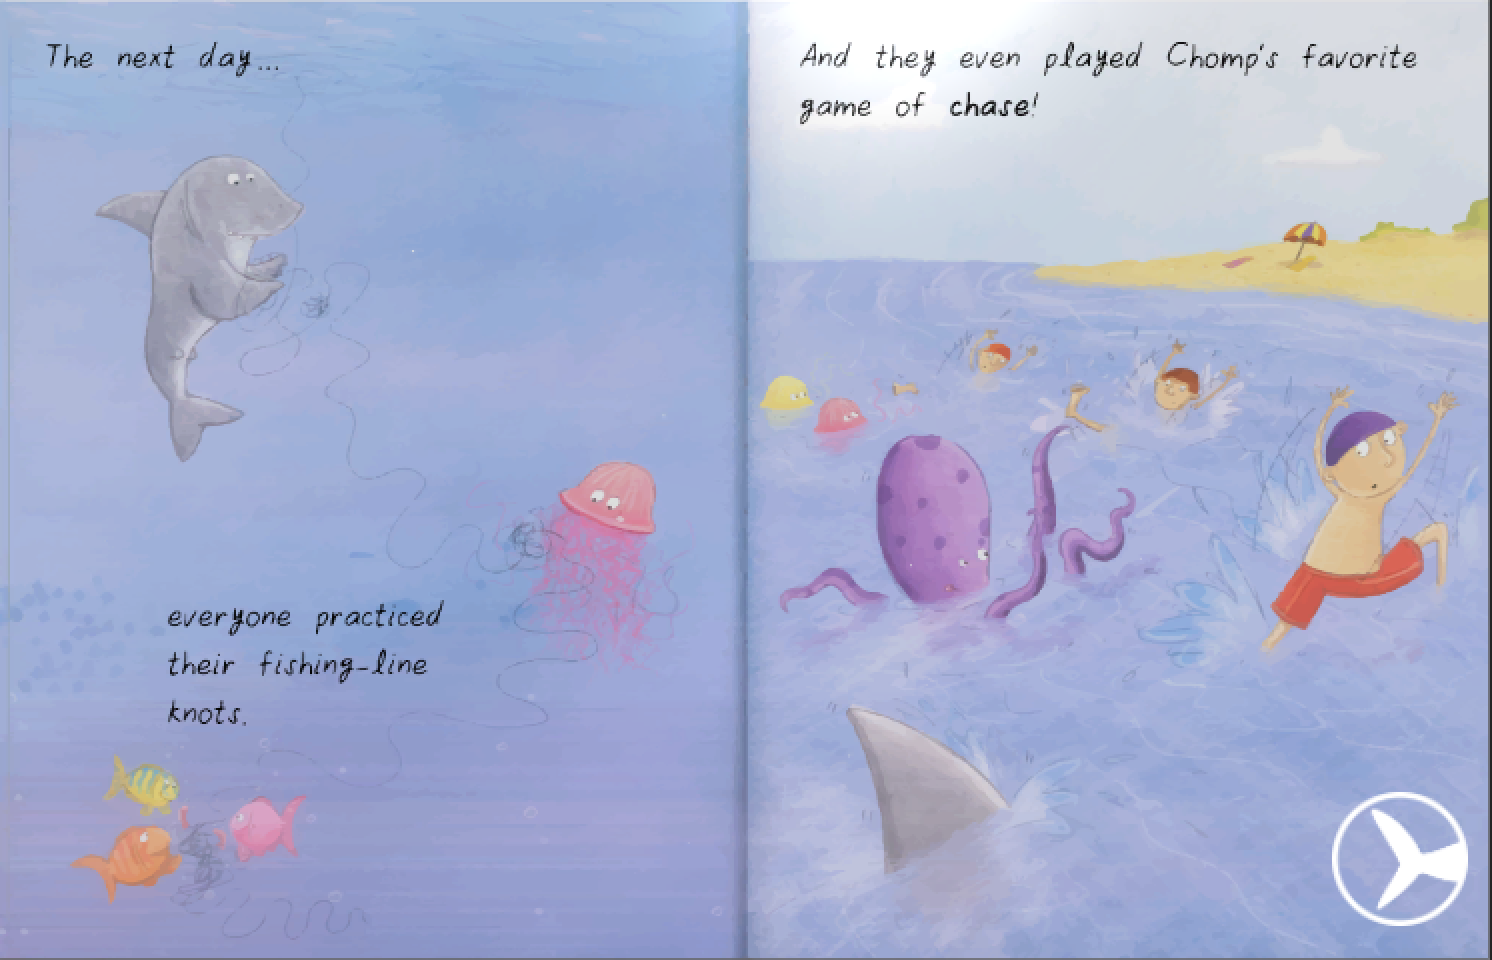
\includegraphics[width=2.5in]{figures/exp2_screencaps/17.png} &
% 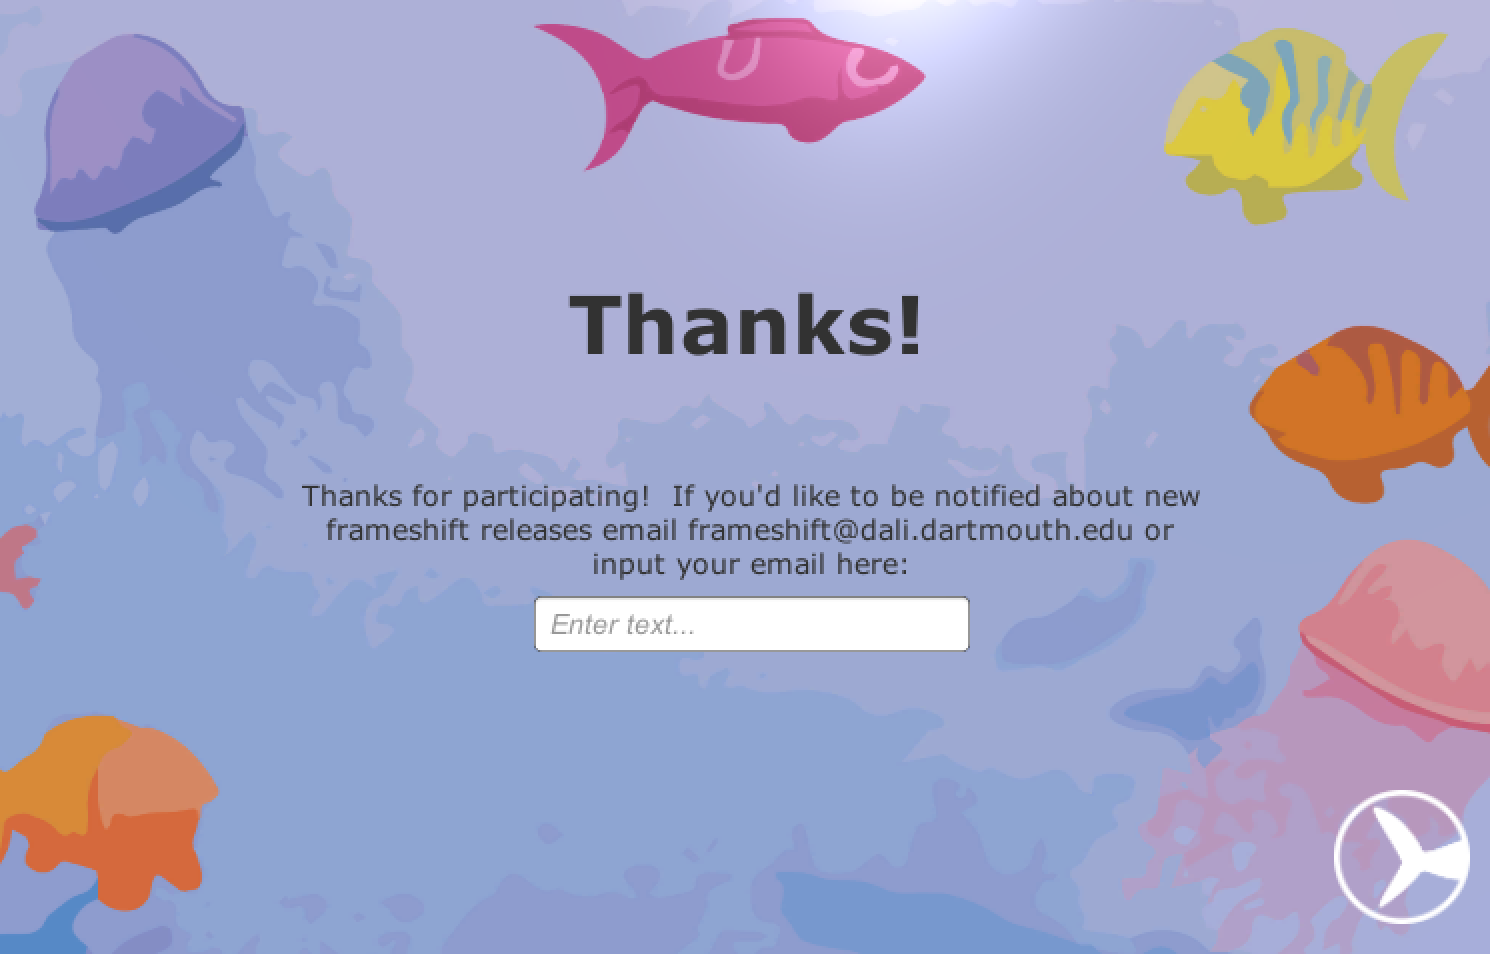
\includegraphics[width=2.5in]{figures/exp2_screencaps/18.png}
% \end{array}$
% \end{center}
% \caption{Trial images from User Study 2, ctd.}
% \end{figure}





